\begin{frame}
\frametitle{Formulation GD / Construction}
\vfill
Étapes de construction de la formulation GD :
\scalebox{0.8}{\begin{minipage}{1.25\textwidth}
\begin{enumerate}[(i)]
\item \textbf{Formulation faible} (fonction test) du problème d'évolution avec \textbf{conditions aux limites} ;
\item Prise en compte des \textbf{discontinuités} de la solution en appliquant la \textbf{condition de saut} ;
\item \textbf{Formulation locale} aux mailles (fonction test nulle en-dehors) ;
\item \textbf{Intégration par parties} (Green) afin de transférer la dérivation spatiale sur la fonction test.
\end{enumerate}
\end{minipage}}
%\vfill
\vskip+1em
\begin{columns}%[c]
\column{0.7\textwidth}
Nous obtenons alors la formulation GD du problème :
\scalebox{0.9}{\begin{minipage}{1.11\textwidth}
\begin{align*}
	\mathcal{H} &= \lbrace
		f \in \mathrm{L}^2(\PbEsp) :
		\forall \L \in \Mesh,
		f_{\vert \L} \in \mathcal{C}^1(\Adh{\L})
	\rbrace , \\
	\W &\in \mathcal{C}^1(\PbTps,\mathcal{H}^\NC) :
	\forall \L \in \Mesh, \forall \psi \in \mathcal{C}^1(\Adh{\L}), \\
	0 &= \int_{\L} \Ptl{t} \At \W \psi d\x
	- \int_{\L} \Aidi \psi \W d\x
	+ \int_{\Bord{\L} \cap \Bord{\PbEsp}}
		(\Aini + \MatB) \W \psi ds \\
	&+ \int_{\Bord{\L} \setminus \Bord{\PbEsp}}
		(\Pos{\Aini} \W_\L + \Neg{\Aini} \W_\R) \psi ds .
\end{align*}
\end{minipage}}
\column{0.3\textwidth}
\begin{figure}
	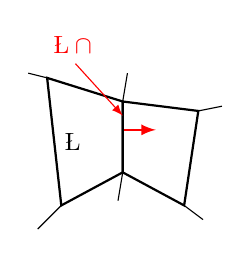
\begin{tikzpicture}[scale=0.6]
		\draw [arrows={-latex},thick,red] (2,2.6)
			-- node[red, midway, below] {\small$\n$} (2.7,2.6); % normal
		\draw [thick] (0.7,1) -- node[midway, right] {\small$\L$} (0.4,3.7)
			-- (2,3.2) -- (2,1.7) -- cycle; % polygon L
		\draw [thick] (2,1.7) -- (2,3.2) -- (3.6,3)
			-- node[midway, left] {\small$\R$} (3.3,1) -- cycle; % polygon R
		\draw [arrows={-latex},red] (1,4) node[above,red] {\small$\Bord{\L} \cap \Bord{\R}$}
			-- (2,2.9); % flèche interface
		\draw (0.7,1) -- (0.2,0.5); % arêtes sortantes
		\draw (0.4,3.7) -- (0,3.8);
		\draw (2,3.2) -- (2.1,3.8);
		\draw (3.6,3) -- (4.1,3.1);
		\draw (3.3,1) -- (3.7,0.7);
		\draw (2,1.7) -- (1.9,1.1);
	\end{tikzpicture}
\end{figure}
\end{columns}
\vfill
\begin{block}{Théorème}
	La méthode est stable si en tout point du bord
	la matrice $\frac{1}{2} \Aini + \MatB$ est positive.
\end{block}
\vfill
\end{frame}

